\chapter{Evolución, resultados y costes}
\label{chap:resultados}

\drop{E}{}n este capítulo se hará un repaso completo a la evolución del proyecto, destacando cada uno de los problemas que han aparecido durante el periodo de desarrollo, así como, la solución que se ha propuesto. De igual manera, se discutirán los resultados que se han obtenido al plantear dos casos de estudio para comprobar el funcionamiento del sistema. Por último, se realizará un desglose de los costes que ha tenido la elaboración del \acs{TFG}.

\section{Evolución}
\label{sec:evolucion}

En Julio de 2015, el artífice de este proyecto comenzó a concentrarse, desde el grupo de investigación ORETO, en el \textbf{desarrollo de un sistema de coordinación de \acs{UAV}s en situaciones de catástrofe}.

Cabe destacar la \textbf{complejidad de trabajar, desarrollar y depender de varios componentes hardware}. Como se muestra seguidamente, en prácticamente todas las fases ha ocurrido algún tipo de inconveniente que dificulta y ralentiza considerablemente el progreso del proyecto. Esto se debe a que en muchas ocasiones es necesario adquirir repuestos nuevos, cuyo envío se demora, y, por lo tanto, los tiempos de desarrollo incrementan.

A continuación, se disgregan en detalle cada una de las fases o periodos de desarrollo del proyecto. 

\begin{figure}[!h]
\begin{center}
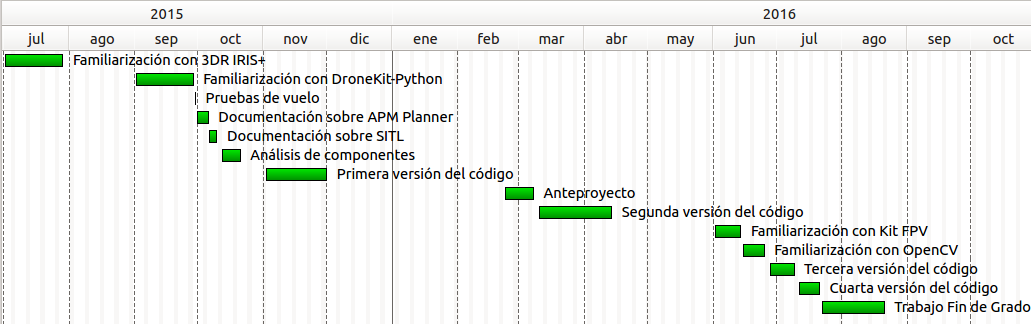
\includegraphics[width=1\textwidth]{/gantt.png}
\caption[Diagrama de distribución de tiempo por tareas en el \acs{TFG}]{Diagrama de distribución de tiempo por tareas en el \acs{TFG}}
\label{fig:gantt}
\end{center}
\end{figure}

\subsection{Fase 0: Julio 2015 - Octubre 2015}
\label{sec:primeraetapa}

En esta primera etapa, el autor debió \textbf{familiarizarse} con el componente fundamental de este proyecto, el dron 3DR IRIS+ y su entorno de desarrollo DroneKit-Python. Se realizaron \textbf{pruebas de simulación}, con código de ejemplo proporcionado por 3D Robotics. También, se hicieron \textbf{pruebas de vuelo} automáticas, en el Instituto de Tecnologías y Sistemas de Información, con el 3DR IRIS+ y la estación de control de tierra APM Planner.

Se profundizó en el estudio de APM Planner y \acs{SITL}, llevando a cabo documentos que sirvieran para dar los primeros pasos en estas plataformas.

Como última parte de esta primera etapa, se realizó un \textbf{análisis de los componentes que se necesitan} y que debían comprarse para llevar a cabo el desarrollo del proyecto. Entre otros se acordó la compra de una cámara GoPro HERO y un kit \acs{FPV}.

Entre los \textbf{problemas producidos} durante esta etapa se encuentra:
\begin{itemize}
\item \textbf{Sistema radiocontrol FlySky FS-TH9X defectuoso}: la palanca correspondiente al \textit{pitch} y al \textit{roll}, con la que se le indica al dron la dirección a la que debe moverse, llegó dañada en el envío. Esto provocaba que el dron ejecutara siempre vuelos hacia la izquierda.\\ La \textbf{solución propuesta} fue reenviar el sistema radiocontrol a 3D Robotics para ser reemplazado. El envío se realizó en Septiembre y no fue recibido de nuevo hasta Noviembre, lo que supuso dos meses sin poder trabajar con el 3DR IRIS+.
\item \textbf{Frecuencia errónea en la telemetría}: el 3DR IRIS+ cuenta con dos modelos disponibles: uno para el uso en Estados Unidos y otro para el uso en el resto del mundo. La diferencia, entre uno y otro, es la frecuencia a la que funciona la telemetría, ya que en Estados Unidos la banda que utiliza es 915 mHz y en el resto del mundo 433 mHz. En este caso, el dron fue adquirido por error con la banda de frecuencia de Estados Unidos, que en España está ocupada por el sistema de telefonía móvil \acs{GSM}. Esto provocaba una serie de interferencias, en el sistema de telemetría, que desembocaban en una lentitud considerable a la hora de cargar los parámetros del 3DR IRIS+ en la estación de control de tierra. Además, no era posible llevar a cabo la conexión con el dron real mediante esta telemetría.\\ La \textbf{solución} a este problema fue comprar una nueva telemetría que funcionara a 433 mHz.
\end{itemize}

\subsection{Fase 1: Noviembre 2015 - Febrero 2016}
\label{sec:segundaetapa}

Meses más tarde, en Noviembre de 2015 se comenzó a desarrollar la \textbf{primera versión del código}. En esta primera versión, se diseñó el sistema, mediante reuniones con David Vallejo, y se implementó el esqueleto de código que ha sido utilizado y mejorado a lo largo del proyecto. 

La primera versión del código contaba con el \textit{Coordinador}, el \textit{Proxy Dron} y el \textit{Dron}. En él, los «waypoints» eran ordenados por prioridad, divididos en listas, que dependían del número de drones que hubiera disponibles, y asignados al vehículo que le correspondiera. Es decir, no se realizaba ningún tipo de coordinación, simplemente todos los puntos de interés eran repartidos, respetando la prioridad, entre él número de vehículos existentes.

Durante el mes de Diciembre y el mes de Enero, se procedió a \textbf{pausar el proyecto} debido a los exámenes finales del primer cuatrimestre. 

Una vez que el periodo de exámenes terminó, se comenzó a \textbf{elaborar el Anteproyecto} en el mes de Febrero.

Entre los \textbf{problemas producidos} durante esta etapa se encuentra:
\begin{itemize}
\item \textbf{Hilos accediendo a recursos compartidos}: al hacer uso de hilos y ejecutar misiones con más de un dron, los vehículos se creaban en el mismo puerto UDP. Este inconveniente ocasionaba que todos los vehículos volaran hacia los mismos puntos de interés, haciendo inservible el empleo de más de un dron en el sistema. \\ La \textbf{solución} a este problema fue utilizar \textit{locks}, como método de sincronización, en el momento en el que se produce la conexión con el dron.
\end{itemize}

\subsection{Fase 2: Marzo 2016 - Mayo 2016}
\label{sec:terceraetapa}

El 8 de Marzo se \textbf{completó la documentación del Anteproyecto} y fue \textbf{enviado} a la Comisión de Trabajos de Fin de Grado. La Comisión de Trabajos de Fin de Grado \textbf{aceptó el Anteproyecto} el 17 de Marzo de 2016.

Tras finalizar el Anteproyecto, el mes de Marzo y Abril comprendió el \textbf{desarrollo de la segunda versión} del proyecto.

En la segunda versión, se modificó la manera en que las misiones son asignadas, puesto que se introdujo el concepto de \textbf{coordinación entre drones}. Se decidió que los puntos de interés se adjudicaran a vehículos que son detectados en un estado ocioso o desocupado. De esta manera, se consiguió mejorar la productividad y el rendimiento del sistema, debido a que anteriormente un vehículo que terminaba de recorrer los «waypoints» que se le habían asignado, no colaboraba con el resto de drones en la misión. 

Además se \textbf{cambió el orden en el que se ejecutaban las operaciones de asignación de puntos de interés y de conexión} con el vehículo. Antes, los puntos de interés eran asignados a vehículos aun no conectados, lo que ocasionaba que si la conexión a un vehículo, al que se le había designado un punto de interés de alta prioridad, tardaba en realizarse, este punto de interés podría ser pasado por alto por otro vehículo cuya conexión haya sido más rápida. De forma que, se estaría incumpliendo el modelo de prioridades del sistema.

Durante el mes de Mayo se volvió a \textbf{detener el desarrollo del proyecto} a causa de los exámenes finales del segundo cuatrimestre.

Entre los \textbf{problemas producidos} durante esta etapa se encuentra:
\begin{itemize}
\item \textbf{Rotura de las patas del dron}: al efectuar el aterrizaje, tras uno de los vuelos de prueba, se parte una de las patas del dron. Esto imposibilita el uso del dron hasta tener piezas de repuesto, dado que el vehículo no dispone de una plataforma segura para el aterrizaje. \\ La \textbf{solución} a este problema fue comprar un pack de patas de repuesto para el 3DR IRIS+, pero en vista de que los pedidos de 3D Robotics tardan en llegar más de un mes, se decidió hacer uso de la impresora 3D, que existe en la Escuela Superior de Informática, para fabricar cuatro patas nuevas que permitieran volar el dron mientras los repuestos eran enviados. 
\end{itemize}

\subsection{Fase 3: Junio 2016 - Septiembre 2016}
\label{sec:cuartaetapa}

Considerando que la coordinación de \acs{UAV}s en situaciones de emergencia ha sido resuelta, con las versiones desarrolladas previamente, en esta etapa se procedió a incorporar los procedimientos para poder \textbf{capturar imágenes} que posteriormente sean \textbf{analizadas}.

Lo primero fue \textbf{familiarizarse con el kit \acs{FPV} y la biblioteca OpenCV}. Ejemplos de código, proporcionados al instalar OpenCV, fueron ejecutados y se grabaron vídeos de prueba hasta comprender que funciones eran necesarias para añadir esta funcionalidad al código del proyecto.

Se realizó una tercera versión, en la que entra en juego el \textit{Sistema FPV}, en la que se grababan las imágenes que procedían de la cámara equipada en el vehículo. Adicionalmente, se estipuló parametrizar el periodo de tiempo, en segundos, cada el que se toma una captura de pantalla de la grabación.

Por último, para realizar la cuarta y última versión del sistema fue necesario entender el funcionamiento de Google Cloud Vision \acs{API}. En la última versión del sistema, se integró el módulo de análisis de imágenes, en el que las capturas de pantalla son examinadas y se muestran por pantalla los resultados obtenidos.

Se decide entregar el \acs{TFG} en Septiembre, por lo que, el mes de Julio y Agosto fue dedicado a documentar el proyecto. Con la entrega del \acs{TFG} el proyecto se considera cerrado en Septiembre de 2016.

Entre los \textbf{problemas producidos} durante esta etapa se encuentra:
\begin{itemize}
\item \textbf{Placa de Tarot T-2D Gimbal estropeada}: mientras se llevaban a cabo pruebas de vuelo, en las que se recogían imágenes, la placa de la gimbal resultó dañada. Se trató de un problema grave, puesto que, no es posible conseguir una grabación de vídeo estable sin ella. \\ La \textbf{solución} a este problema fue comprar una nueva placa, junto con unos nuevos motores estabilizadores.
\item \textbf{Baterías para el sistema \acs{FPV} deterioradas}: para que el sistema \acs{FPV} funcione, es necesario contar con dos baterias de 1300 mAh, una para el transmisor y otra para el receptor. Dos de las tres baterías de las que se disponía, sufrieron desperfectos y dejaron de cargar. Por lo tanto, el sistema \acs{FPV} quedó inoperativo. \\ La \textbf{solución} a este problema fue comprar nuevas baterías de 1300 mAh.
\end{itemize}
 
\section{Caso de estudio}

\section{Costes}

Es complicado dar un valor exacto al coste del proyecto, a causa de que los ciclos de trabajo no han sido constantes durante todo el desarrollo del sistema. Varias circunstancias han contribuido a que se detenga o se aminore, en varias ocasiones, la actividad del proyecto. Algunos de estas circunstancias son:

\begin{itemize}
\item Fases en las que se debía esperar la llegada de algún repuesto para poder hacer uso del sistema.
\item Periodos de exámenes.
\item Fechas en las que se debían entregar prácticas y trabajos de distintas asignaturas.
\item Compaginación con contrato deportivo.
\end{itemize}  

Por esta razón, se hará una estimación en la que se tase el coste del proyecto atendiendo a las siguientes pautas:

\begin{itemize}
\item Sueldo en Europa de un programador en Python que cuenta con una experiencia de 1 a 4 años: según Payscale \footnote{\url{http://www.payscale.com}} el salario se encuentra establecido en \textbf{14 euros por hora}.
\item El proyecto ha supuesto 13 meses de desarrollo, de los cuales se atribuyen \textbf{8 meses como productivos} al descontar los periodos de exámenes, las vacaciones y la espera hasta la llegada de repuestos.
\item Se establece un horario laboral de jornada completa, es decir, \textbf{40 horas semanales}.
\item El coste de los dispositivos hardware necesarios para elaborar el \acs{TFG}: la suma de la compra de todos los componentes asciende a \textbf{1.845,21 euros} (Ver Anexo).
\end{itemize}

Así pues, \textbf{el coste del proyecto se estima en 28.725,21 euros}.

% Local Variables:
% coding: utf-8
% mode: latex
% mode: flyspell
% ispell-local-dictionary: "castellano8"
% End:
